\documentclass[border=2pt]{standalone}

\usepackage{amsmath} 
\usepackage{cancel}
\usepackage{fancyhdr}
\usepackage{xfrac}
\usepackage{amssymb}
\usepackage{subfig}
\usepackage{graphicx}
\usepackage{wrapfig}
\usepackage{minted}
\usepackage{tikz}
\usepackage{pgfplots}
\usepackage{hyperref}
\usetikzlibrary{decorations.pathreplacing,calligraphy}
\usepgfplotslibrary{fillbetween}
\usetikzlibrary{positioning}

\begin{document}

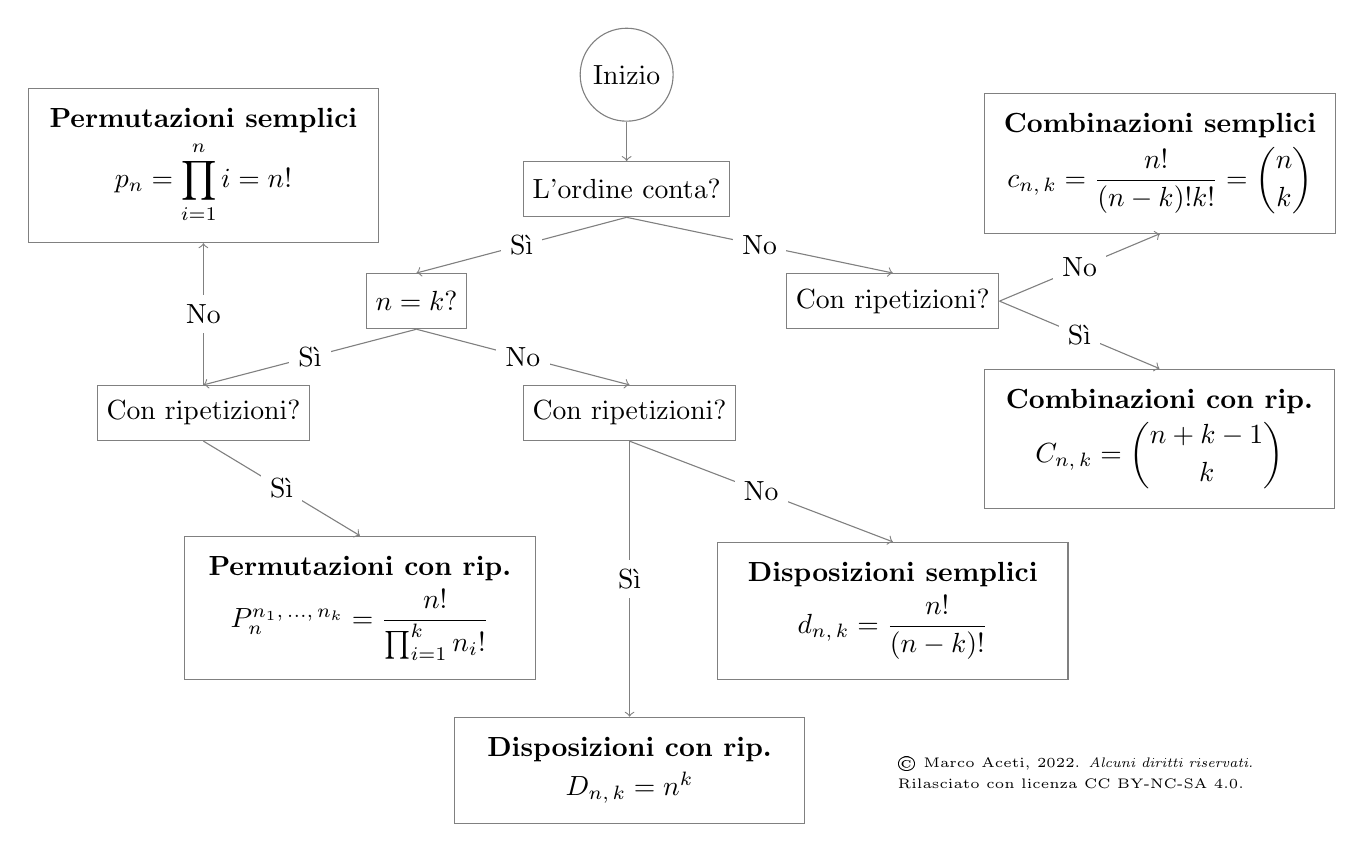
\begin{tikzpicture}[
round/.style={circle, draw=gray, minimum size=10mm},
rect/.style={rectangle, draw=gray, minimum size=7mm},
bigrect/.style={rectangle, draw=gray, minimum width=4.45cm, inner sep=2.5mm},
]

\node[round] (start) {Inizio};
\node[rect] (order) [below=5mm of start] {L'ordine conta?};
\node[rect] (nk) [below left=10mm of order] {$n=k$?};
\node[rect] (rip1) [below right=10mm of order] {Con ripetizioni?};

\node[rect] (rip2) [below left=10mm of nk] {Con ripetizioni?};
\node[bigrect] (perm_s) [above=18mm of rip2, align=center] {\textbf{Permutazioni semplici} \\[0.8mm]
$p_n = \displaystyle \prod_{i=1}^n i = n!$
};
\node[bigrect] (perm_r) [below right=12mm and -16mm of rip2, align=center] {\textbf{Permutazioni con rip.} \\[0.8mm]
$P_n^{n_1, \, \dots, \, n_k} = \displaystyle \frac {n!}{\prod_{i=1}^k n_i!}$
};

\node[bigrect] (comb_s) [above right=5mm and -2mm of rip1, align=center] {\textbf{Combinazioni semplici} \\[0.8mm]
$c_{n, \, k} = \dfrac{n!}{(n-k)!k!} = \displaystyle \binom{n}{k}$
};
\node[bigrect] (comb_r) [below right=5mm and -2mm of rip1, align=center] {\textbf{Combinazioni con rip.} \\[0.8mm]
$C_{n, \, k} = \displaystyle \binom{n+k-1}{k}$
};
\node[rect] (rip3) [below right=10mm of nk] {Con ripetizioni?};
\node[bigrect] (disp_s) [below=27mm of rip1, align=center] {\textbf{Disposizioni semplici} \\[0.8mm]
$d_{n, \, k} = \dfrac{n!}{(n-k)!}$
};
\node[bigrect] (disp_r) [below=35mm of rip3, align=center] {\textbf{Disposizioni con rip.} \\[0.8mm]
$D_{n, \, k} = n^k$
};

\draw[gray, ->] (start.south) -- (order.north);
\draw[gray, ->] (order.south) -- (nk.north) node[black, midway, fill=white] {Sì};
\draw[gray, ->] (order.south) -- (rip1.north) node[black, midway, fill=white] {No};

\draw[gray, ->] (rip2.north) -- (perm_s.south) node[black, midway, fill=white] {No};
\draw[gray, ->] (rip2.south) -- (perm_r.north) node[black, midway, fill=white] {Sì};

\draw[gray, ->] (nk.south) -- (rip2.north) node[black, midway, fill=white] {Sì};
\draw[gray, ->] (nk.south) -- (rip3.north) node[black, midway, fill=white] {No};

\draw[gray, ->] (rip3.south) -- (disp_r.north) node[black, midway, fill=white] {Sì};
\draw[gray, ->] (rip3.south) -- (disp_s.north) node[black, midway, fill=white] {No};

\draw[gray, ->] (rip1.east) -- (comb_s.south) node[black, midway, fill=white] {No};
\draw[gray, ->] (rip1.east) -- (comb_r.north) node[black, midway, fill=white] {Sì};

\node[] at (5.75, -8.75) [align=left] {\tiny{\textcopyright \ Marco Aceti, 2022. \textit{Alcuni diritti riservati.}} 
};
\node[] at (5.655, -9.00) [align=left] {\tiny{
\tiny{Rilasciato con licenza CC BY-NC-SA 4.0.}
}};
\end{tikzpicture}


\end{document}
